
\makequotation{It is practically impossible to teach good programming to
  students that have had a prior exposure to BASIC: as potential
  programmers they are mentally mutilated beyond hope of
  regeneration.}{Edsger W. Dijkstra, Turing Award winner~\cite{dijkstra-truths}}

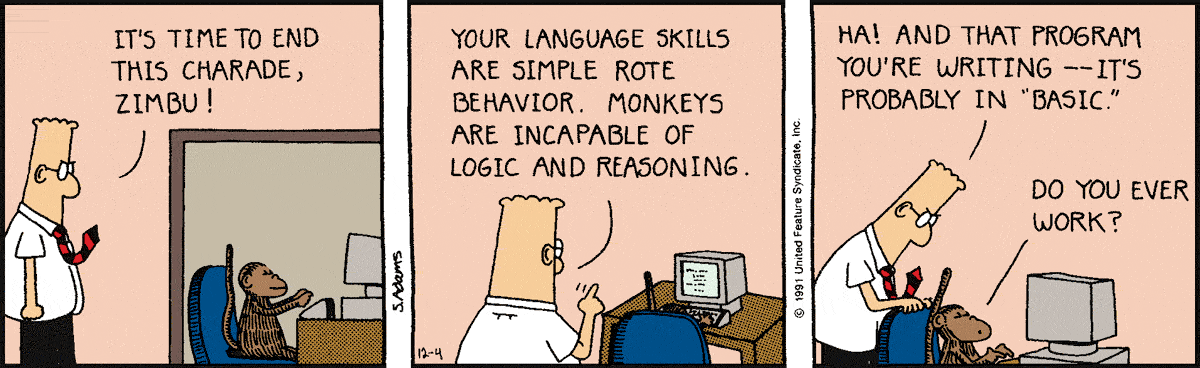
\includegraphics[width=\textwidth]{figs/dilbert-1991-12-04.png}

Much has been written over the decades about the democratization of
computers thanks to Moore's Law, but what has been overlooked is that up
until the consumer Internet appeared in around 1995, BASIC was present
at every milestone, and played a pivotal role in empowering generations
of programmers.
Yet BASIC is probably one of the most maligned programming languages
to achieve widespread use.

BASIC's co-creators have defended the language~\cite{backtobasic} on the
grounds that the 
``hacks'' for which BASIC is often criticized were absent from 
 their original design, appearing only later in ``unauthorized''
 adaptations for PCs.
%% This defense seems doubtful, since the original language did include
%% \T{GO~TO}, which Dijkstra famously railed
%% against~\cite{goto_considered_harmful}.
Science fiction author David Brin mounts a different
defense~\cite{why_johnny_cant_code}: 
for all its flaws, BASIC
was sufficiently nonthreatening to introduce an entire generation of
newbies to the joy of programming\footnote{\href{http://quitebasic.com}{QuiteBASIC.com}, an
in-browser BASIC environment developed in response to Brin's article, is
a good proxy for the ``old school BASIC'' Brin praises.}%
, whereas today's more expressive
(if better-designed) languages for higher-powered 
platforms, such as Python or Perl, may scare beginners away.
Of course, Python represents 
nearly a quarter-century of language design experience since BASIC's birth.

Regardless, the criticisms are misguided.
The goal of BASIC's creators was to expose as many non-programmers as
possible to programming.
While today's world-class universities boast that over 90\% of all
undergraduates are exposed to introductory programming, Dartmouth had
achieved this by 1971~\cite{man_and_computer} by implementing the
farsighted vision of BASIC's creators.
And with the help of a wide cast of characters who wittingly or
unwittingly played key roles in BASIC's subsequent dissemination---Bob
Albrecht, David Ahl, Paul Allen, Dennis Allison, Bill Gates, Chuck
Peddle, Ed Roberts, Li-Chen Wang, Steve Wozniak, and the companies and
institutions where they worked---BASIC then introduced an entire generation
of hobbyist programmers to programming.
If along the way we learned bad habits that structured languages tried to
break, we also learned computational thinking.

It's time the true story of BASIC's influence was told.
